
\documentclass[tikz,border=7pt]{standalone}
\usepackage[utf8]{inputenc}
\usepackage[T1]{fontenc}
\usepackage{amsmath}
\usepackage{xcolor}
\usetikzlibrary{arrows.meta,calc,angles,quotes,patterns,positioning}
\definecolor{brand}{HTML}{1E3A8A}
\definecolor{brandtwo}{HTML}{2563EB}
\definecolor{accentred}{HTML}{EF4444}
\definecolor{accentgreen}{HTML}{16A34A}
\definecolor{accentorange}{HTML}{F59E0B}
\definecolor{muted}{HTML}{64748B}
\definecolor{lightblue}{HTML}{EEF6FF}
\tikzset{force/.style={-{Latex[length=3mm]}, line width=1.15pt}, axis/.style={-{Latex[length=2mm]}, line width=.8pt, color=muted}, body/.style={draw=brandtwo, fill=lightblue, line width=1pt, rounded corners=2pt}, lab/.style={font=\small, text=brand}, sml/.style={font=\scriptsize, text=muted}}
\begin{document}

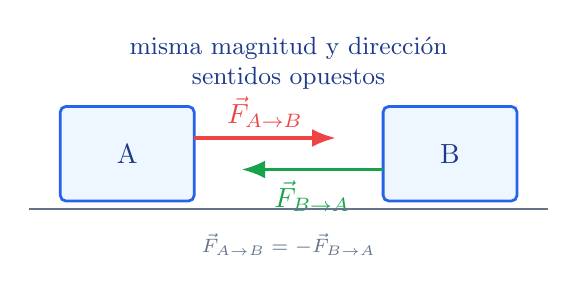
\begin{tikzpicture}[scale=1]
\draw[body] (0,0) rectangle (1.7,1.2); \draw[body] (4.1,0) rectangle (5.8,1.2);
\node[text=brand] at (.85,.6) {A}; \node[text=brand] at (4.95,.6) {B};
\draw[force, color=accentred] (1.7,.8)--(3.5,.8) node[midway,above] {$\vec F_{A\to B}$};
\draw[force, color=accentgreen] (4.1,.4)--(2.3,.4) node[midway,below] {$\vec F_{B\to A}$};
\draw[thick, color=muted] (-.4,-.1)--(6.2,-.1);
\node[lab, align=center] at (2.9,1.75) {misma magnitud y dirección\\sentidos opuestos};
\node[sml] at (2.9,-.55) {$\vec F_{A\to B}=-\vec F_{B\to A}$};
\end{tikzpicture}

\end{document}